\section{Component Types}
The definition of software components in UML 2.0 includes the definition of a component type, which is not elaborated in more detail as discussed above.

\begin{figure}
\centering
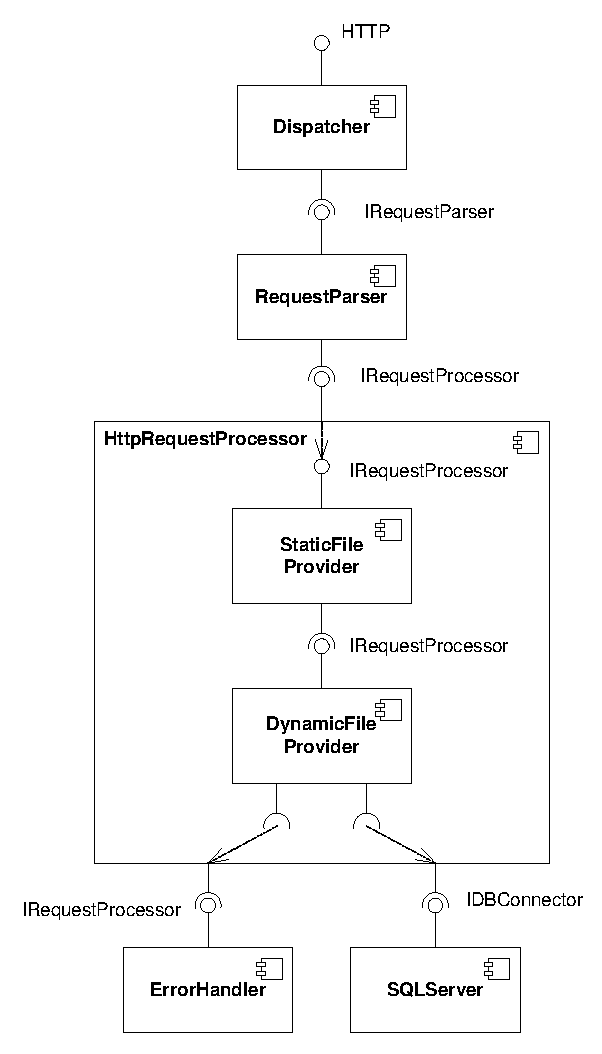
\includegraphics[width=3.3in]{example/WebserverComponents}
\caption{Component Model of a Web Server.}
\label{fig:WebserverComponents}
\end{figure}

Figure \ref{fig:WebserverComponents} shows the architecture of a simple web server. 


The components \texttt{StaticFileProvider} and \texttt{HttpRequestProcessor} provide and require the same set of interfaces.

\begin{figure}
\centering
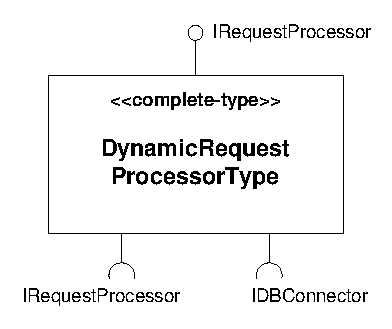
\includegraphics[scale=1.0]{example/DynamicRequestProcessorType}
\caption{A component type used at different points in the web server.}
\label{fig:DynamicRequestProcessorType}
\end{figure}

This is not the only Type that is used in the component model of the web server.

\begin{figure}
\centering
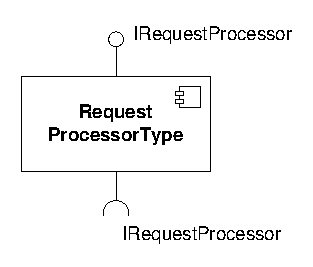
\includegraphics[scale=1.0]{example/RequestProcessorType}
\caption{Another component type used in the web server.}
\label{fig:RequestProcessorType}
\end{figure}

So, some components provide the same interfaces, but require different services to complete their task.
Distinguish between Provided and Complete types. Both have their advantages. They are defined by substitutability. 

The development process of a component is not fixed to both types of a component, but is an evolutionary process.
During Software architecture design, there is no clear border between both types.

The stepwise completion of a component specification leads to different interpretations of required interfaces.
-	can be used, but there can be more (provided type interpretation)
-	can only be used (complete type)
-	has to be used in a predefined fashion (not considered in our case, example: information has to be stored in a database, so the interface of the database must be used.

Conformance between Provided and Complete Types.
